\documentclass[tikz,border=10pt]{standalone}
\usetikzlibrary{calc}
\usetikzlibrary{arrows.meta}
\begin{document}

\newcommand{\basejet}[1][]{

  \begin{scope}
    \draw (0,1) circle(0.3cm and 0.07cm);
  \end{scope}
  \draw[thick,gray,->,line cap =round] (0.00,0.04) -- node[left,font=\footnotesize] {} (90:1.4);
  \draw[gray,->,line cap =round] (0.00,0.02) -- node[left,font=\footnotesize] {} (80:1.3);
  \draw[gray,->,line cap =round] (0.00,0.02) -- node[left,font=\footnotesize] {} (100:1.3);

  \begin{scope}
    \clip (-1,0) rectangle (1,1);
    \draw (0,1) circle(0.3cm and 0.07cm);
  \end{scope}
  \draw[line cap =round] (0.00,0.02) -- (0.3,1);
  \draw[line cap =round] (0.00,0.02) -- (-0.3,1);
  #1
}

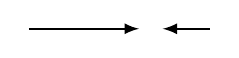
\begin{tikzpicture}

  \draw[thick,-{latex[length=3mm]}] (-1.5,0) -- (-0.1,0);
  \draw[thick,-{latex[length=3mm]}] (0.8,0) -- (0.2,0);

  \begin{scope}[shift={(0.0,0.0)}]
    \begin{scope}[rotate=-60]
      \basejet
    \end{scope}
    \begin{scope}[rotate=240]
      \basejet
    \end{scope}
  \end{scope}



\end{tikzpicture}
\end{document}
